\section{Analysis of ALT}
In this section we study the various components of ALT, and provide insights into their impact on generalization. 
\begin{figure*}
    \centering
    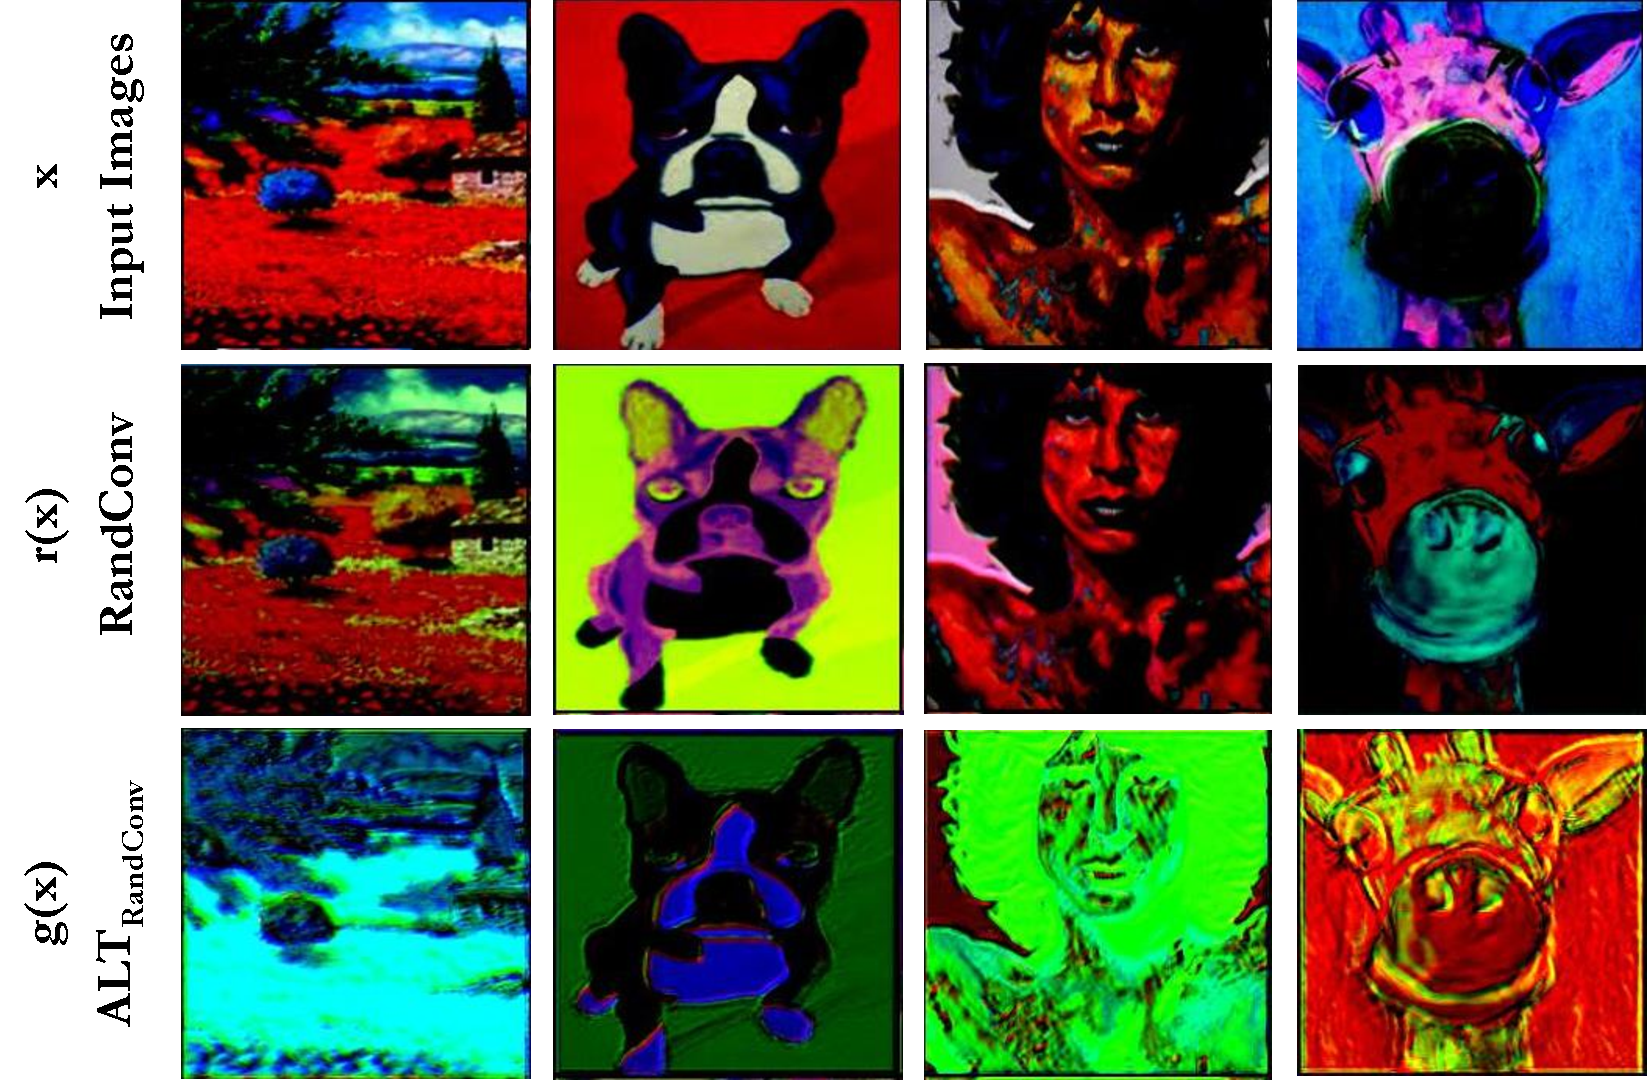
\includegraphics[width=0.48\linewidth]{alt/figures/viz_randconv_alt.pdf}
    \quad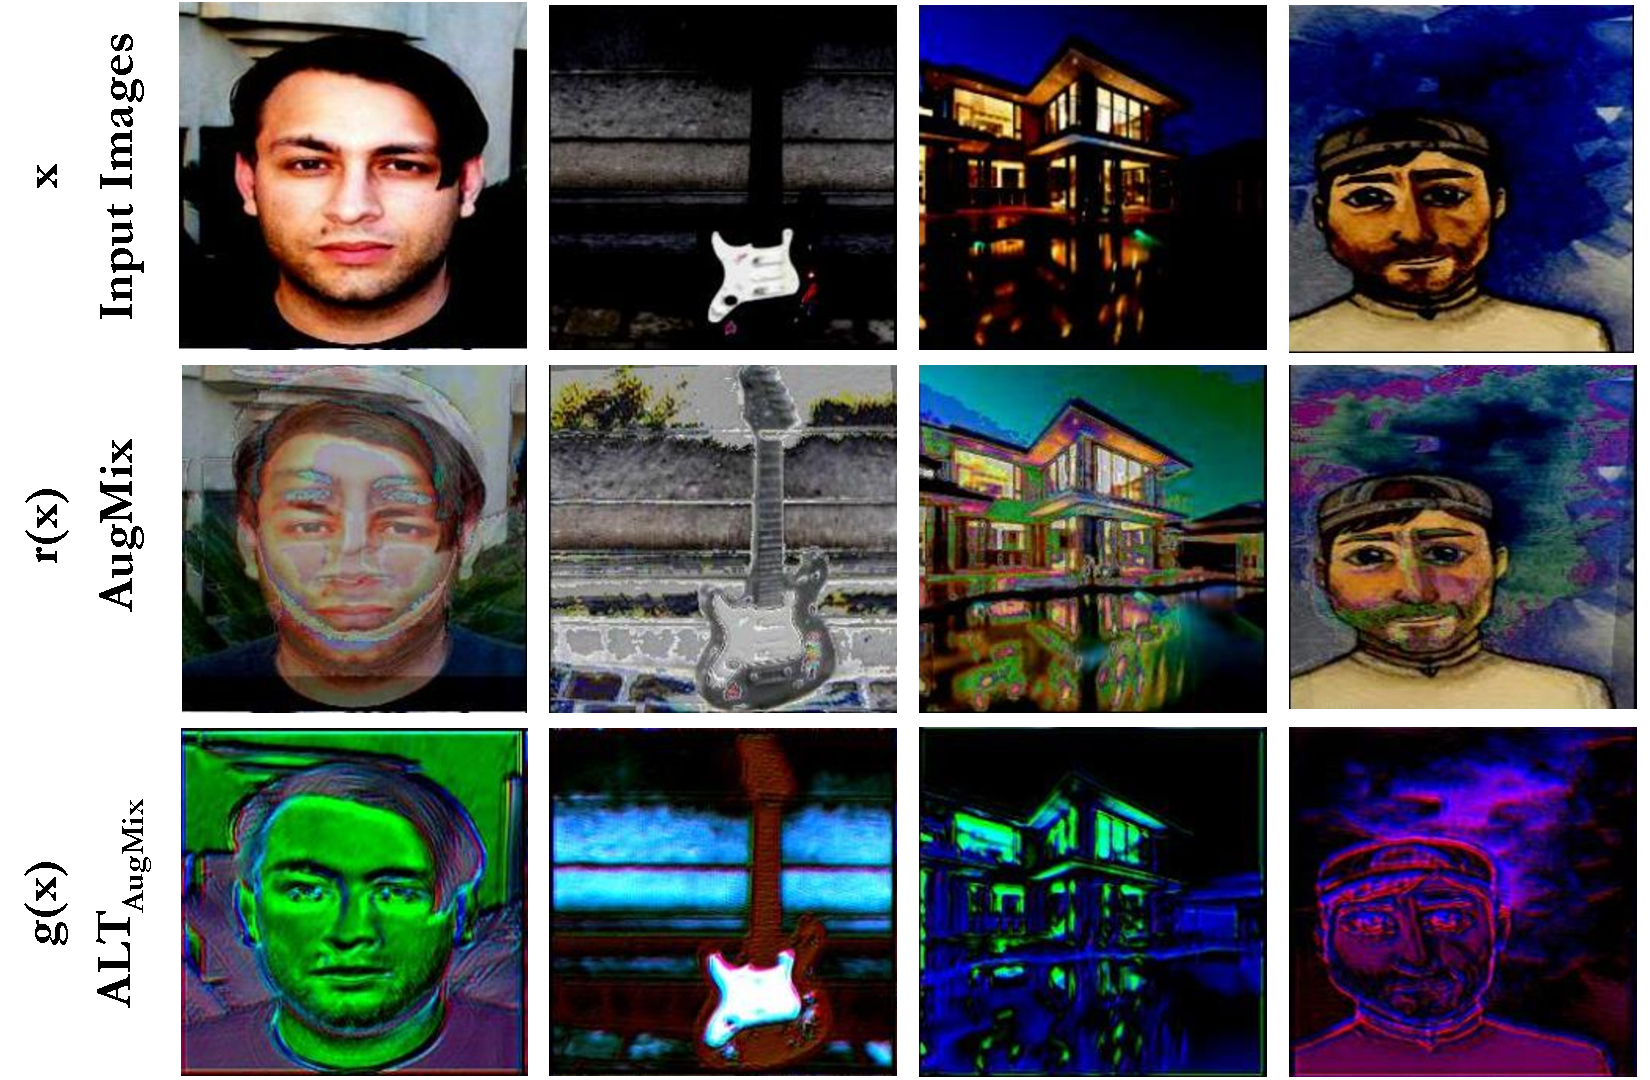
\includegraphics[width=0.48\linewidth]{alt/figures/viz_augmix_alt.pdf}
    \caption{Comparison of images transformed by data augmentation techniques RandConv \textit{(left)} and AugMix \textit{(right)} and their combination with ALT (ALT$_{RandConv}$ and ALT$_{AugMix}$), 
    illustrating the wide range of transformations learned by ALT.}
    \label{fig:viz_augs}
\end{figure*}

\paragraph{ALT is better than na\"ive diversity} Our first big insight is that ALT without an explicit diversity module still outperforms all the top performing methods across the benchmarks we evaluated on, indicating that learned adversarial transformations are a powerful way to train classifiers for generalization. They include diversity (achieved through random initializations) and adversarial images that help expose the classifier to large distribution shifts. Our next observation is that ALT makes the choice of diversity module fairly arbitrary. We see this effect on multiple benchmarks -- for example, on the Digits benchmark shown in  \Cref{tab:results_digits}, AugMix has a relatively poor generalization performance when compared with the baseline ERM whereas ALT$_{Augmix}$ achieves state of the art. This is again seen in the Office-Home benchmark shown in \Cref{tab:results_officehome}, where RandConv is worse than ERM, but ALT$_{RandConv}$ is the best performing method. We show examples of the image transformations learned with ALT in Figure~\ref{fig:viz_augs}, and it is clear that ALT achieves far more diverse and larger transformations of the input images than either AugMix or RandConv.

% - basically talk about diversity alone (Augmix/RC) -- see some boost, but varying results on each benchmark.
% MNIST -- augmix boosts by 1\% barely, but big jump for RandConv.
% On PACS and OfficeHome, AugMix is better than RandConv.
% - ALT without diversity is better than Diversity alone
% - ALT can better adapt its diversity when combined with RandConv and Augmix -- the combination and interplay between the adversarial cost and consistency, is key.


\paragraph{ALT Hyperparameters.}
The four main hyper-parameters that control ALT are: the consistency coefficient $\lambda_{KL}$ in Equation~\ref{alt:eq:L_KL} which decides the proportion between the classifier loss and KL-divergence consistency between transformations, 
number of adversarial steps and learning rate in the adversarial maximization of Equation~\ref{alt:eq:adv_max}, and the diversity weight $w_r$ which controls the interaction between the diversity module $r()$ and the adversary network $g()$ in Equation~\ref{alt:eq:p_mix}.
We investigate the effect of each of these on domain generalization accuracy in Figure~\ref{fig:digits_hp}.
The first plot shows that the consistency coefficient $\lambda_{KL}$ is impactful and a higher value leads to better generalization.
However at $\lambda_{KL}=1.0$ the accuracy degenerates to random performance; this is expected as the classifier loss gets $1-\lambda_{KL}{=}0$ weight.
From the second and third plots, we observe that an optimal value exists around 20 adversarial steps and learning rate of $1e{-}5$.
There is a fast drop in generalization at higher learning rates.
Increasing the diversity weight also leads to increase in generalization, however at $w_r{=}2$ the performance drops and corresponds to "diversity only" settings.
Clearly, the adversarial component is a critical factor that causes improvements in generalization.

\begin{table}[t]
    \centering
    % \small
    \begin{tabular}{@{}lccc@{}}
        \toprule
        \textbf{Architecture} & \textbf{Digits Average} & \textbf{PACS Average} \\
        \midrule
        FCN (2 layers) & 72.75 & 63.40 \\
        FCN (3 layers) & 73.74 & 63.92\\
        FCN (4 layers) & 74.10 & 64.41 \\
        FCN (5 layers) & 73.87 & 64.20 \\
        FCN (6 layers) & 74.15 & 63.78\\
        % ResNetGen-6~\cite{johnson2016perceptual} & \\
        % UNet-10~\cite{ronneberger2015u} & \\
        \bottomrule
    \end{tabular}
    \caption{Effect of the architecture of the adversity network $g$ on average domain generalization on the PACS and Digits benchmarks.}
    \label{tab:gvars}
\end{table}

% \begin{table}[t]
%     \centering
%     \begin{tabular}{cc}
%         \toprule
%         \textbf{Method}     & \textbf{DG Avg.}\\
%         \midrule
%         RandConv            & \\
%         AugMix              & 59.56\\
%         ALT$_{RandConv}$    & \\
%         ALT$_{AugMix}$      & \\
%         ALT$_{none}$        & \\
%         \bottomrule
%     \end{tabular}
%     \caption{PACS DG Average}
%     \label{tab:ablation_hd}
% \end{table}

\paragraph{Complexity of Adversary Network.}
In our experiments on the benchmark datasets we have used a simple fully convolutional network (FCN) with 5 convolutional layers.
We conduct additional analysis to understand how this choice affects generalization performance, and compare performance when using between 2 and 6 convolutional layers.
% We compare FCN with number of layers between 2 and 6.
% and two additional architectures -- U-Net-10~\citep{ronneberger2015u} with 5 downsampling and 5 upsampling operations (UNet-10) and a ResNet based generator (ResNetGen-6) with 3 downsampling and 3 upsampling operations. operations~\citep{johnson2016perceptual}.
% Note that the UNet and ResNet generators are considerably more sophisticated than FCN, and contain bottleneck architectures and skip connections.
We reuse all other training settings from our benchmark model $ALT_{RandConv}$ on both Digits and PACS.
For PACS, we observe that all ALT models compared are better than previous baselines including AugMix and RandConv.
For Digits, we observe that performance of ALT with a 2-layer $g$ is close to RandConv, and is greater than all previous baselines for higher depth of the network.
Increasing the number of layers, i.e., increasing the complexity of the adversary network leads to better performance upto 5 layers, even with the same learning rate.

% \paragraph{Qualitative Comparison of Diverse Augmentations}

% \begin{figure}[t]
%     \centering
%     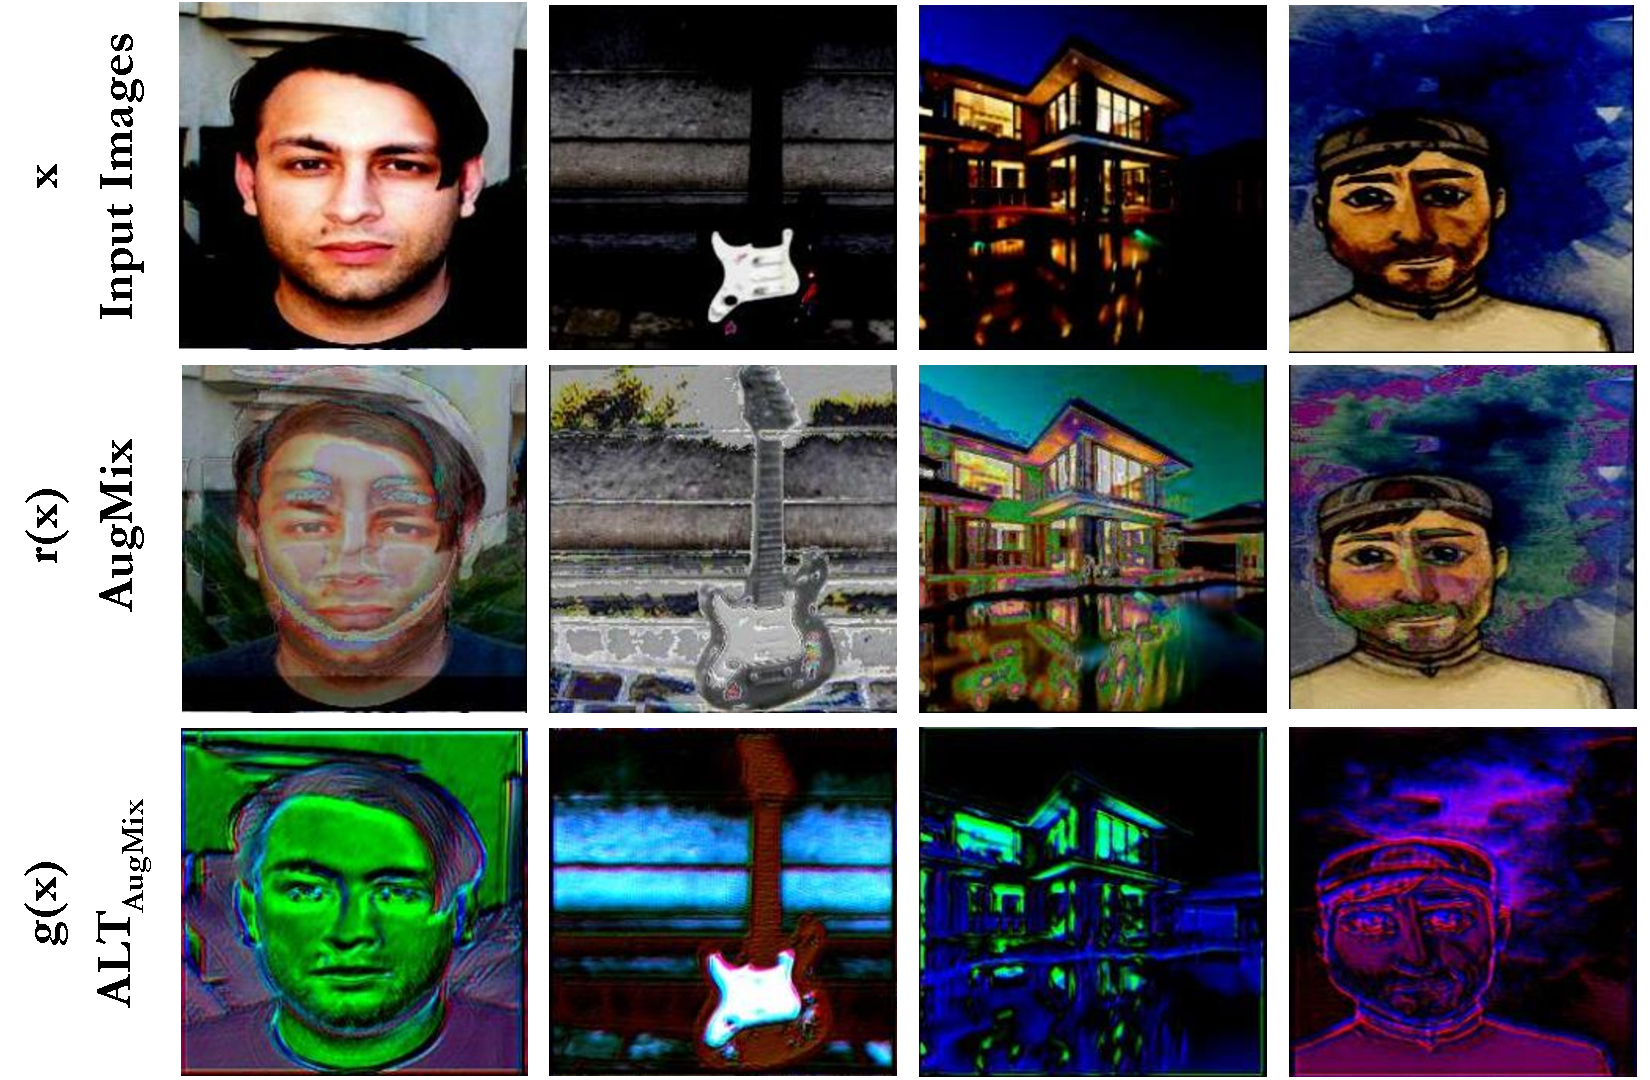
\includegraphics[width=\linewidth]{alt/figures/viz_augmix_alt.pdf}
%     \caption{Comparison of transformed images for AugMix and ALT$_{AugMix}$.}
%     \label{fig:viz_augmix}
% \end{figure}
% In Figure~\ref{fig:viz_augs} we illustrate the difference between the augmentations generated by RandConv, AugMix, ALT$_{g-only}$, ALT$_{RandConv}$ and ALT$_{AugMix}$.
